\documentclass{ximera}

%\usepackage{todonotes}

\newcommand{\todo}{}

\usepackage{esint} % for \oiint
\ifxake%%https://math.meta.stackexchange.com/questions/9973/how-do-you-render-a-closed-surface-double-integral
\renewcommand{\oiint}{{\large\bigcirc}\kern-1.56em\iint}
\fi


\graphicspath{
  {./}
  {ximeraTutorial/}
  {basicPhilosophy/}
  {functionsOfSeveralVariables/}
  {normalVectors/}
  {lagrangeMultipliers/}
  {vectorFields/}
  {greensTheorem/}
  {shapeOfThingsToCome/}
  {dotProducts/}
  {partialDerivativesAndTheGradientVector/}
  {../productAndQuotientRules/exercises/}
  {../normalVectors/exercisesParametricPlots/}
  {../continuityOfFunctionsOfSeveralVariables/exercises/}
  {../partialDerivativesAndTheGradientVector/exercises/}
  {../directionalDerivativeAndChainRule/exercises/}
  {../commonCoordinates/exercisesCylindricalCoordinates/}
  {../commonCoordinates/exercisesSphericalCoordinates/}
  {../greensTheorem/exercisesCurlAndLineIntegrals/}
  {../greensTheorem/exercisesDivergenceAndLineIntegrals/}
  {../shapeOfThingsToCome/exercisesDivergenceTheorem/}
  {../greensTheorem/}
  {../shapeOfThingsToCome/}
  {../separableDifferentialEquations/exercises/}
}

\newcommand{\mooculus}{\textsf{\textbf{MOOC}\textnormal{\textsf{ULUS}}}}

\usepackage{tkz-euclide}\usepackage{tikz}
\usepackage{tikz-cd}
\usetikzlibrary{arrows}
\tikzset{>=stealth,commutative diagrams/.cd,
  arrow style=tikz,diagrams={>=stealth}} %% cool arrow head
\tikzset{shorten <>/.style={ shorten >=#1, shorten <=#1 } } %% allows shorter vectors

\usetikzlibrary{backgrounds} %% for boxes around graphs
\usetikzlibrary{shapes,positioning}  %% Clouds and stars
\usetikzlibrary{matrix} %% for matrix
\usepackage{pgfplots}
\usepgfplotslibrary{polar} %% for polar plots
\usepgfplotslibrary{fillbetween} %% to shade area between curves in TikZ
\usetkzobj{all}
\usepackage[makeroom]{cancel} %% for strike outs
%\usepackage{mathtools} %% for pretty underbrace % Breaks Ximera
%\usepackage{multicol}
\usepackage{pgffor} %% required for integral for loops



%% http://tex.stackexchange.com/questions/66490/drawing-a-tikz-arc-specifying-the-center
%% Draws beach ball
\tikzset{pics/carc/.style args={#1:#2:#3}{code={\draw[pic actions] (#1:#3) arc(#1:#2:#3);}}}



\usepackage{array}
\setlength{\extrarowheight}{+.1cm}
\newdimen\digitwidth
\settowidth\digitwidth{9}
\def\divrule#1#2{
\noalign{\moveright#1\digitwidth
\vbox{\hrule width#2\digitwidth}}}





\newcommand{\RR}{\mathbb R}
\newcommand{\R}{\mathbb R}
\newcommand{\N}{\mathbb N}
\newcommand{\Z}{\mathbb Z}

\newcommand{\sagemath}{\textsf{SageMath}}


%\renewcommand{\d}{\,d\!}
\renewcommand{\d}{\mathop{}\!d}
\newcommand{\dd}[2][]{\frac{\d #1}{\d #2}}
\newcommand{\pp}[2][]{\frac{\partial #1}{\partial #2}}
\renewcommand{\l}{\ell}
\newcommand{\ddx}{\frac{d}{\d x}}

\newcommand{\zeroOverZero}{\ensuremath{\boldsymbol{\tfrac{0}{0}}}}
\newcommand{\inftyOverInfty}{\ensuremath{\boldsymbol{\tfrac{\infty}{\infty}}}}
\newcommand{\zeroOverInfty}{\ensuremath{\boldsymbol{\tfrac{0}{\infty}}}}
\newcommand{\zeroTimesInfty}{\ensuremath{\small\boldsymbol{0\cdot \infty}}}
\newcommand{\inftyMinusInfty}{\ensuremath{\small\boldsymbol{\infty - \infty}}}
\newcommand{\oneToInfty}{\ensuremath{\boldsymbol{1^\infty}}}
\newcommand{\zeroToZero}{\ensuremath{\boldsymbol{0^0}}}
\newcommand{\inftyToZero}{\ensuremath{\boldsymbol{\infty^0}}}



\newcommand{\numOverZero}{\ensuremath{\boldsymbol{\tfrac{\#}{0}}}}
\newcommand{\dfn}{\textbf}
%\newcommand{\unit}{\,\mathrm}
\newcommand{\unit}{\mathop{}\!\mathrm}
\newcommand{\eval}[1]{\bigg[ #1 \bigg]}
\newcommand{\seq}[1]{\left( #1 \right)}
\renewcommand{\epsilon}{\varepsilon}
\renewcommand{\phi}{\varphi}


\renewcommand{\iff}{\Leftrightarrow}

\DeclareMathOperator{\arccot}{arccot}
\DeclareMathOperator{\arcsec}{arcsec}
\DeclareMathOperator{\arccsc}{arccsc}
\DeclareMathOperator{\si}{Si}
\DeclareMathOperator{\scal}{scal}
\DeclareMathOperator{\sign}{sign}


%% \newcommand{\tightoverset}[2]{% for arrow vec
%%   \mathop{#2}\limits^{\vbox to -.5ex{\kern-0.75ex\hbox{$#1$}\vss}}}
\newcommand{\arrowvec}[1]{{\overset{\rightharpoonup}{#1}}}
%\renewcommand{\vec}[1]{\arrowvec{\mathbf{#1}}}
\renewcommand{\vec}[1]{{\overset{\boldsymbol{\rightharpoonup}}{\mathbf{#1}}}}
\DeclareMathOperator{\proj}{\mathbf{proj}}
\newcommand{\veci}{{\boldsymbol{\hat{\imath}}}}
\newcommand{\vecj}{{\boldsymbol{\hat{\jmath}}}}
\newcommand{\veck}{{\boldsymbol{\hat{k}}}}
\newcommand{\vecl}{\vec{\boldsymbol{\l}}}
\newcommand{\uvec}[1]{\mathbf{\hat{#1}}}
\newcommand{\utan}{\mathbf{\hat{t}}}
\newcommand{\unormal}{\mathbf{\hat{n}}}
\newcommand{\ubinormal}{\mathbf{\hat{b}}}

\newcommand{\dotp}{\bullet}
\newcommand{\cross}{\boldsymbol\times}
\newcommand{\grad}{\boldsymbol\nabla}
\newcommand{\divergence}{\grad\dotp}
\newcommand{\curl}{\grad\cross}
%\DeclareMathOperator{\divergence}{divergence}
%\DeclareMathOperator{\curl}[1]{\grad\cross #1}
\newcommand{\lto}{\mathop{\longrightarrow\,}\limits}

\renewcommand{\bar}{\overline}

\colorlet{textColor}{black}
\colorlet{background}{white}
\colorlet{penColor}{blue!50!black} % Color of a curve in a plot
\colorlet{penColor2}{red!50!black}% Color of a curve in a plot
\colorlet{penColor3}{red!50!blue} % Color of a curve in a plot
\colorlet{penColor4}{green!50!black} % Color of a curve in a plot
\colorlet{penColor5}{orange!80!black} % Color of a curve in a plot
\colorlet{penColor6}{yellow!70!black} % Color of a curve in a plot
\colorlet{fill1}{penColor!20} % Color of fill in a plot
\colorlet{fill2}{penColor2!20} % Color of fill in a plot
\colorlet{fillp}{fill1} % Color of positive area
\colorlet{filln}{penColor2!20} % Color of negative area
\colorlet{fill3}{penColor3!20} % Fill
\colorlet{fill4}{penColor4!20} % Fill
\colorlet{fill5}{penColor5!20} % Fill
\colorlet{gridColor}{gray!50} % Color of grid in a plot

\newcommand{\surfaceColor}{violet}
\newcommand{\surfaceColorTwo}{redyellow}
\newcommand{\sliceColor}{greenyellow}




\pgfmathdeclarefunction{gauss}{2}{% gives gaussian
  \pgfmathparse{1/(#2*sqrt(2*pi))*exp(-((x-#1)^2)/(2*#2^2))}%
}


%%%%%%%%%%%%%
%% Vectors
%%%%%%%%%%%%%

%% Simple horiz vectors
\renewcommand{\vector}[1]{\left\langle #1\right\rangle}


%% %% Complex Horiz Vectors with angle brackets
%% \makeatletter
%% \renewcommand{\vector}[2][ , ]{\left\langle%
%%   \def\nextitem{\def\nextitem{#1}}%
%%   \@for \el:=#2\do{\nextitem\el}\right\rangle%
%% }
%% \makeatother

%% %% Vertical Vectors
%% \def\vector#1{\begin{bmatrix}\vecListA#1,,\end{bmatrix}}
%% \def\vecListA#1,{\if,#1,\else #1\cr \expandafter \vecListA \fi}

%%%%%%%%%%%%%
%% End of vectors
%%%%%%%%%%%%%

%\newcommand{\fullwidth}{}
%\newcommand{\normalwidth}{}



%% makes a snazzy t-chart for evaluating functions
%\newenvironment{tchart}{\rowcolors{2}{}{background!90!textColor}\array}{\endarray}

%%This is to help with formatting on future title pages.
\newenvironment{sectionOutcomes}{}{}



%% Flowchart stuff
%\tikzstyle{startstop} = [rectangle, rounded corners, minimum width=3cm, minimum height=1cm,text centered, draw=black]
%\tikzstyle{question} = [rectangle, minimum width=3cm, minimum height=1cm, text centered, draw=black]
%\tikzstyle{decision} = [trapezium, trapezium left angle=70, trapezium right angle=110, minimum width=3cm, minimum height=1cm, text centered, draw=black]
%\tikzstyle{question} = [rectangle, rounded corners, minimum width=3cm, minimum height=1cm,text centered, draw=black]
%\tikzstyle{process} = [rectangle, minimum width=3cm, minimum height=1cm, text centered, draw=black]
%\tikzstyle{decision} = [trapezium, trapezium left angle=70, trapezium right angle=110, minimum width=3cm, minimum height=1cm, text centered, draw=black]


\title[Dig-In]{Maximums and minimums}

\outcome{Define a critical point.}
\outcome{Find critical points.}
\outcome{Define absolute maximum and absolute minimum.}
\outcome{Find the absolute max or min of a continuous function on a closed interval.}
\outcome{Define local maximum and local minimum.}
\outcome{Compare and contrast local and absolute maxima and minima.}
\outcome{Identify situations in which an absolute maximum or minimum is guaranteed.}
\outcome{Classify critical points.}
\outcome{State the First Derivative Test.}
\outcome{Apply the First Derivative Test.}
\outcome{State the Second Derivative Test.}
\outcome{Apply the Second Derivative Test.}
\outcome{Define inflection points.}
\outcome{Find inflection points.}
  
\begin{document}
\begin{abstract}
We use derivatives to help locate extrema.  
\end{abstract}
\maketitle


Whether we are interested in a function as a purely mathematical
object or in connection with some application to the real world, it is
often useful to know what the graph of the function looks like. We can
obtain a good picture of the graph using certain crucial information
provided by derivatives of the function.

\section{Extrema}

Local \textit{extrema} of a function are points on the graph where the
$y$-coordinate is larger (or smaller) than all other $y$-coordinates
on the graph at points ``close to'' $(x,y)$. 

\begin{definition}\hfil\index{maximum/minimum!local}
\begin{enumerate}
\item A function $f$ has a \dfn{local maximum} at $x=a$, if $f(a)\ge
  f(x)$ for every $x$ in some open interval I containing $a$.
\item A function $f$ has a \dfn{local minimum} at $x=a$, if $f(a)\le
  f(x)$ for every $x$  in some open interval I containing $a$.
\end{enumerate}
A \dfn{local extremum}\index{extremum!local} is either a local
maximum or a local minimum.
\end{definition}

%% \begin{question} BADBAD I want this question
%%   True or false: ``All absolute extrema are also local extrema.''
%%   \begin{multipleChoice}
%%     \choice[correct]{true}
%%     \choice{false}
%%   \end{multipleChoice}
%%   \begin{feedback}
%%     All global extrema are local extrema.
%%   \end{feedback}
%% \end{question}
In our next example, we clarify the definition of a local minimum.
\begin{example}
Consider the graph of a function $f$:
\begin{image}
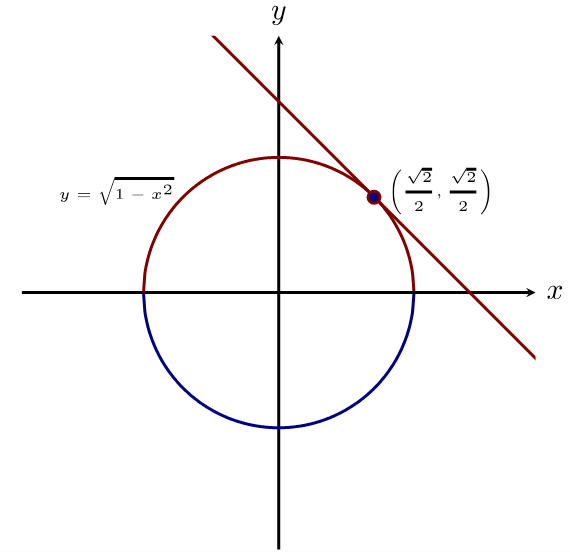
\includegraphics{0.png}
%% \caption{A plot of $f(x) = x^3-4x^2+3x$ and $f'(x) = 3x^2-8x+3$.}
%% \label{figure:x^3-4x^2+3x}
\end{image}
Identify the local extrema of $f$ and give an explanation.
\begin{explanation}
In the figure above the function $f$ has a local minimum at,
\[
a=\answer[given]{1},
\]
because were able to find an \textbf{open} interval $I$ (marked in the
figure) that contains the number
\[
a=\answer[given]{1},
\]
and for all numbers $x$ in $I$ the following statement is true:
 \[
f\left(\answer[given]{1}\right)\le f\left(\answer[given]{x}\right).
\]
\end{explanation}
\end{example}

Local maximum and minimum points are quite distinctive on the graph of
a function, and are, therefore, useful in understanding the shape of the
graph. In many applied problems we want to find the largest or
smallest value that a function achieves (for example, we might want
to find the minimum cost at which some task can be performed) and so
identifying maximum and minimum points will be useful for applied
problems as well.



\section{Critical points}

Consider the graph of the function $f$.
\begin{image}
  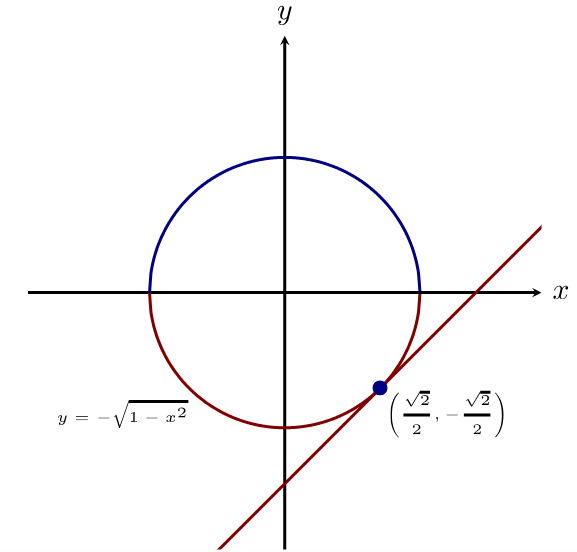
\includegraphics{1.png}
\end{image}
The function $f$  has four local extremums: at  $x=-4$, $x=-2$, $x=0$ and $x=4$.
Notice that the function $f$ is \textbf{not differentiable} at  $x=-4$ and  $x=-2$.
Notice that $f'(0)=0$ and $f'(4)=0$.

After this example, the following theorem should not come as a surprise. 


\begin{theorem}[Fermat's Theorem]\index{Fermat's Theorem}\label{theorem:fermat}
If $f$ has a local extremum at $x=a$ and $f$ is differentiable
at $a$, then $f'(a)=0$.
\end{theorem}
\begin{question}
  Does Fermat's Theorem say that if $f'(a) = 0$, then $f$ has a local
  extrema at $x=a$?
  \begin{multipleChoice}
    \choice{yes}
    \choice[correct]{no}
  \end{multipleChoice}
  \begin{feedback}
    Consider $f(x) = x^3$, $f'(0) = 0$, but $f$ does not have a local
    maximum or minimum at $x=0$.
  \end{feedback}
\end{question}


Fermat's Theorem says that the only points at which a function can
have a local maximum or minimum are points at which the derivative is
zero or the derivative is undefined. As an illustration of the first scenario, consider the plots of $f(x) = x^3-4.5x^2+6x$ and $f'(x) =
3x^2-9x+6$.
\begin{image}
  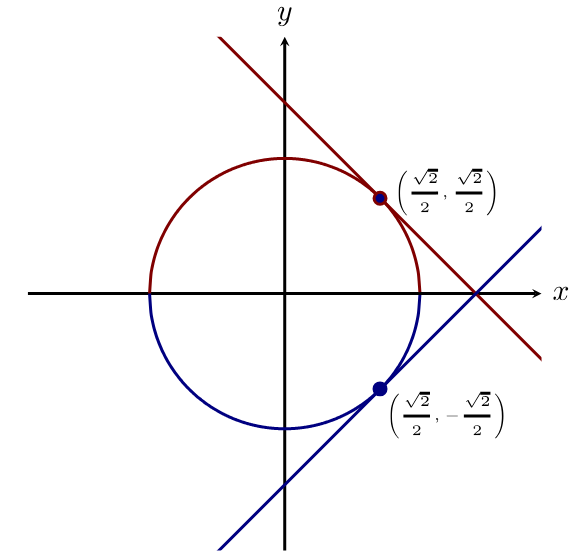
\includegraphics{2.png}
%% \caption{A plot of $f(x) = x^3-4x^2+3x$ and $f'(x) = 3x^2-8x+3$.}
%% \label{figure:x^3-4x^2+3x}
\end{image}
\begin{question}
 Make a correct choice that completes the sentence below. \\
 
  At the point $(1,f(1))$, the  function $f$ has 

  \begin{multipleChoice}
    \choice[correct]{a local maximum}
    \choice{a local minimum}
    \choice{no local extremum}
  \end{multipleChoice}
  \end{question}
  \begin{question}
Select the correct statement.
  \begin{multipleChoice}
    \choice{$f'(1)$ is undefined}
    \choice{$f'(1)>0$}
    \choice[correct]{$f'(1)=0$}
     \choice{$f'(1)<0$}
  \end{multipleChoice}
\end{question}
\begin{question}
 Make a correct choice that completes the sentence below. \\
 
  At the point $(1.5,f(1.5))$, the  function $f$ has 

  \begin{multipleChoice}
    \choice{a local maximum}
    \choice{a local minimum}
    \choice[correct]{no local extremum}
  \end{multipleChoice}
  \end{question}
  \begin{question}
Select the correct statement.
  \begin{multipleChoice}
    \choice{$f'(1.5)$ is undefined}
    \choice{$f'(1.5)>0$}
    \choice{$f'(1.5)=0$}
     \choice[correct]{$f'(1.5)<0$}
  \end{multipleChoice}
\end{question}

\begin{question}
 Make a correct choice that completes the sentence below. \\
 
  At the point $(2,f(2))$, the  function $f$ has 

  \begin{multipleChoice}
    \choice{a local maximum}
    \choice[correct]{a local minimum}
    \choice{no local extremum}
  \end{multipleChoice}
  \end{question}
  \begin{question}
Select the correct statement.
  \begin{multipleChoice}
    \choice{$f'(2)$ is undefined}
    \choice{$f'(2)>0$}
    \choice[correct]{$f'(2)=0$}
     \choice{$f'(2)<0$}
  \end{multipleChoice}
\end{question}
 As an illustration of the second scenario, consider the plots of $f(x) = x^{2/3}$ and $f'(x) = \frac{2}{3x^{1/3}}$:
\begin{image}
  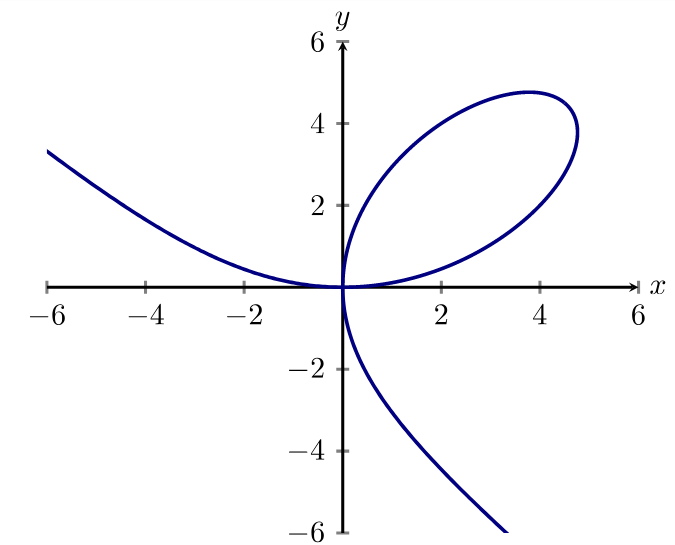
\includegraphics{3.png}
%% \caption{A plot of $f(x) = x^{2/3}$ and $f'(x) = \frac{2}{3x^{1/3}}$.}
%% \label{figure:x^{2/3}}
\end{image}
\begin{question}
 Make a correct choice that completes the sentence below. \\
 
  At the point $(-2,f(-2))$, the  function $f$ has 

  \begin{multipleChoice}
    \choice{a local maximum}
    \choice{a local minimum}
    \choice[correct]{no local extremum}
  \end{multipleChoice}
  \end{question}
  \begin{question}
Select the correct statement.
  \begin{multipleChoice}
    \choice{$f'(-2)$ is undefined}
    \choice{$f'(-2)>0$}
    \choice{$f'(-2)=0$}
     \choice[correct]{$f'(-2)<0$}
  \end{multipleChoice}
\end{question}
\begin{question}
 Make a correct choice that completes the sentence below. \\
 
  At the point $(0,0)$, the  function $f$ has 

  \begin{multipleChoice}
    \choice{a local maximum}
    \choice[correct]{a local minimum}
    \choice{no local extremum}
  \end{multipleChoice}
  \end{question}
  \begin{question}
Select the correct statement.
  \begin{multipleChoice}
    \choice[correct]{$f'(0)$ is undefined}
    \choice{$f'(0)>0$}
    \choice{$f'(0)=0$}
     \choice{$f'(0)<0$}
  \end{multipleChoice}
\end{question}

This brings us to our next definition.

\begin{definition}\index{critical point}
  Assume that a function $f$ is defined on an open interval I that contains a point $a$. The  function $f$ has a \dfn{critical point} at $x=a$ if 
  \[
  f'(a) = 0\qquad\text{or}\qquad \text{$f'(a)$ does not exist.}
  \]
\end{definition}

\begin{warning} 
When looking for local maximum and minimum points, you are likely to
make two sorts of mistakes: 
\begin{itemize}
\item You may forget that a maximum or minimum can occur where the
  derivative does not exist, and so forget to check whether the
  derivative exists everywhere. 
\item You might assume that any place that the derivative is zero is a
  local maximum or minimum point, but this is not true, consider the
  plots of $f(x) = x^3$ and $f'(x) = 3x^2$.
\begin{image}
  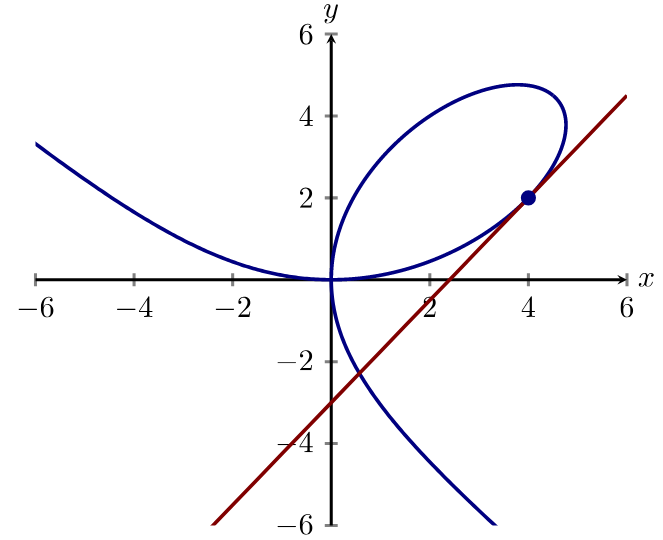
\includegraphics{4.png}
%% \caption{A plot of $f(x) = x^3$ and $f'(x) = 3x^2$. While $f'(0)=0$,
%%   there is neither a maximum nor minimum at $(0,f(0))$.}
%% \label{figure:x^3}
\end{image}
While $f'(0)=0$, there is neither a maximum nor minimum at $x=0$.
\end{itemize}
\end{warning}



Since both local maximum and
local minimum occur at a critical point, when we locate a critical point, we need to determine which, if either,
actually occurs. 
\begin{example}
Find all local maximum and minimum points for the function 
$f(x)=x^3-x$. 
\begin{explanation} 
Write
\[
\ddx f(x)=\answer[given]{3x^2-1}.
\] 
We can easily express  $f'(x)$ as a product of its factors
\[
\ddx
f(x)=3\left(x+\answer[given]{\frac{\sqrt{3}}{3}}\right)\left(x-\answer[given]{\frac{\sqrt{3}}{3}}\right),
\] 
which implies that the function $f$ has only two critical points,
$x=-\frac{\sqrt{3}}{3}$ and $x=\frac{\sqrt{3}}{3}$. Notice that the
derivative $f'(x)$ is a polynomial, and polynomials do not change
signs except possibly at their zeros. This implies that derivative
$f'(x)$ \textbf{does not change the sign} on the intervals
$\left(-\infty,-\frac{\sqrt{3}}{3}\right)$,
$\left(-\frac{\sqrt{3}}{3},\frac{\sqrt{3}}{3}\right)$, and
$\left(\frac{\sqrt{3}}{3},\infty\right)$, because these intervals do not contain
any zeros of $f'(x)$.
 
\begin{question}
Select the correct statement about the sign of $f'(x)$ on the
intervals $\left(-\infty,-\frac{\sqrt{3}}{3}\right)$ and
$\left(-\frac{\sqrt{3}}{3},\frac{\sqrt{3}}{3}\right)$. 
\begin{multipleChoice}
  \choice{$f'(x)>0$ on $\left(-\infty,-\frac{\sqrt{3}}{3}\right)$ and $f'(x)>0$ on $\left(-\frac{\sqrt{3}}{3},\frac{\sqrt{3}}{3}\right)$. }
  \choice[correct]{$f'(x)>0$ on $x$ in $\left(-\infty,-\frac{\sqrt{3}}{3}\right)$ and $f'(x)<0$ on $\left(-\frac{\sqrt{3}}{3},\frac{\sqrt{3}}{3}\right)$. }
  \choice{$f'(x)<0$ on $\left(-\infty,-\frac{\sqrt{3}}{3}\right)$ and $f'(x)>0$ on $\left(-\frac{\sqrt{3}}{3},\frac{\sqrt{3}}{3}\right)$. }
  \choice{$f'(x)<0$ on $\left(-\infty,-\frac{\sqrt{3}}{3}\right)$ and $f'(x)<0$ on $\left(-\frac{\sqrt{3}}{3},\frac{\sqrt{3}}{3}\right)$}
\end{multipleChoice}
  \end{question}
  If we know the sign of the derivative on an interval, we also know whether the function is increasing or decreasing on that interval. This will help us determine whether the function has a local extremum at the critical point  where $x=-\frac{\sqrt{3}}{3}$. \\
  \begin{question}

At the critical point where $x=-\frac{\sqrt{3}}{3}$, the function $f$ has  \\
 
  \begin{multipleChoice}
    \choice{no local extremum, because $f$ is increasing on $\left(-\infty,-\frac{\sqrt{3}}{3}\right)$ and increasing on $\left(-\frac{\sqrt{3}}{3},\frac{\sqrt{3}}{3}\right)$. }
      \choice[correct]{a local maximum, because $f$ is increasing on $\left(-\infty,-\frac{\sqrt{3}}{3}\right)$ and decreasing on $\left(-\frac{\sqrt{3}}{3},\frac{\sqrt{3}}{3}\right)$. }
      \choice{a local minimum, because $f$ is decreasing on $\left(-\infty,-\frac{\sqrt{3}}{3}\right)$ and increasing on $\left(-\frac{\sqrt{3}}{3},\frac{\sqrt{3}}{3}\right)$. }
         \choice{no local extremum, because $f$ is decreasing on $\left(-\infty,-\frac{\sqrt{3}}{3}\right)$ and decreasing on $\left(-\frac{\sqrt{3}}{3},\frac{\sqrt{3}}{3}\right)$. }  \end{multipleChoice}
  \end{question}
  \begin{question}
Select the correct  statement about the sign of $f'(x)$ on the intervals  $\left(-\frac{\sqrt{3}}{3},\frac{\sqrt{3}}{3}\right)$ and  $\left(\frac{\sqrt{3}}{3},\infty\right)$. \\
 
  \begin{multipleChoice}
    \choice{$f'(x)>0$ on $\left(-\frac{\sqrt{3}}{3},\frac{\sqrt{3}}{3}\right)$  and $f'(x)>0$ on $\left(\frac{\sqrt{3}}{3},\infty\right)$.}
    \choice{$f'(x)>0$ on $\left(-\frac{\sqrt{3}}{3},\frac{\sqrt{3}}{3}\right)$ and $f'(x)<0$ on $\left(\frac{\sqrt{3}}{3},\infty\right)$.}
       \choice[correct]{$f'(x)<0$ on   $\left(-\frac{\sqrt{3}}{3},\frac{\sqrt{3}}{3}\right)$  and $f'(x)>0$ on $\left(\frac{\sqrt{3}}{3},\infty\right)$.}
         \choice{$f'(x)<0$ on  $\left(-\frac{\sqrt{3}}{3},\frac{\sqrt{3}}{3}\right)$  and $f'(x)<0$ on $\left(\frac{\sqrt{3}}{3},\infty\right)$.}
  \end{multipleChoice}
  \end{question}
Again, the sign of the derivative on an interval determines whether the function is increasing or decreasing on that interval. This will help us determine whether the function has a local extremum at the critical point  where $x=\frac{\sqrt{3}}{3}$. \\
  \begin{question}

At the critical point where $x=\frac{\sqrt{3}}{3}$, the function $f$ has  \\
 
  \begin{multipleChoice}
    \choice{no local extremum, because $f$ is increasing on $\left(-\frac{\sqrt{3}}{3},\frac{\sqrt{3}}{3}\right)$ and increasing on $\left(\frac{\sqrt{3}}{3},\infty\right)$. }
       \choice{a local maximum, because $f$ is increasing on $\left(-\frac{\sqrt{3}}{3},\frac{\sqrt{3}}{3}\right)$ and decreasing on $\left(\frac{\sqrt{3}}{3},\infty\right)$. }
      \choice[correct]{a local minimum, because $f$ is decreasing on $\left(-\frac{\sqrt{3}}{3},\frac{\sqrt{3}}{3}\right)$ and increasing on $\left(\frac{\sqrt{3}}{3},\infty\right)$. }
        \choice{no local extremum, because $f$ is decreasing on$\left(-\frac{\sqrt{3}}{3},\frac{\sqrt{3}}{3}\right)$ and decreasing on $\left(\frac{\sqrt{3}}{3},\infty\right)$. }
      \end{multipleChoice}
  \end{question}
 Do your answers agree with the graphs of $f$ and $f'$ given in the picture below?
\begin{image}
  \includegraphics{5.png}
%%\caption{A plot of $f(x) = x^3-x$ and $f'(x) = 3x^2-1$.}
%%\label{figure:x^3-x}
\end{image}
\end{explanation}
\end{example}






\section{The first derivative test}

We will further explore and refine the method of the previous section for deciding whether there is a
local maximum or minimum at a critical point.
 Recall that
\begin{itemize}
\item If $f'(x) >0$ on an interval, then $f$ is increasing on that interval.
\item If $f'(x) <0$ on an interval, then $f$ is decreasing on that interval.
\end{itemize}

So how exactly does the derivative tell us whether there is a maximum,
minimum, or neither at a point? Use the \textit{first derivative test}.

\begin{theorem}[First Derivative Test]\index{first derivative test}\label{T:fdt}
Suppose that $f$ is continuous on an interval, and that $f'(a)=0$ for
some value of $a$ in that interval.
\begin{itemize}
\item If $f'(x)>0$ to the left of $a$ and $f'(x)<0$ to the right of
  $a$, then $f(a)$ is a local maximum.
\item If $f'(x)<0$ to the left of $a$ and $f'(x)>0$ to the right of
  $a$, then $f(a)$ is a local minimum.
\item If $f'(x)$ has the same sign to the left and right of $a$,
  then $f(a)$ is not a local extremum.
\end{itemize}
\end{theorem}

\begin{example}\label{E:localextrema}
Consider the function 
\[
f(x) = \frac{x^4}{4}+\frac{x^3}{3}-x^2
\]
Find the intervals on which $f$ is increasing and decreasing and
identify the local extrema of $f$.


\begin{explanation}
Start by computing
\[
\ddx f(x) = \answer[given]{x^3+x^2-2x}.
\]
Now we need to find on what intervals is $f'$ positive and what intervals it is
negative. To do this, solve 
\[
f'(x) = \answer[given]{x^3+x^2-2x} =0.
\]
Factor $f'(x)$
\begin{align*}
f'(x) &= \answer[given]{x^3+x^2-2x} \\
&=x(\answer[given]{x^2+x-2})\\
&=x(x+2)(\answer[given]{x-1}).
\end{align*}
So the critical points (when $f'(x)=0$) are when $x=-2$, $x=0$, and
$x=1$. Since the derivative, $f'(x)$, is a polynomial, it does not change the sign on intervals between its zeros, i.e., between the critical points. Now we can check the sign of $f'(x)$ at some points \textbf{between} the critical points to find
where $f'(x)$ is positive and where negative:
\begin{align*}
  f'(-3)&=\answer[given]{-12},\\
  f'(.5)&=\answer[given]{-0.625},\\
  f'(-1)&=\answer[given]{2},\\
  f'(2)&=\answer[given]{8}.
\end{align*}
From this we can make a sign table:

\begin{image}
  \includegraphics{6.png}
\end{image}

Hence $f$ is increasing on $(-2,0)$ and $(1,\infty)$ and $f$ is
decreasing on $(-\infty,-2)$ and $(0,1)$. Moreover, from the first
derivative test, the local maximum is at $x=0$ while the local minimums
are at $x=-2$ and $x=1$, see the graphs of $f(x) =x^4/4 + x^3/3
-x^2$ and $f'(x) = x^3 + x^2 -2x$.
\begin{image}
  \includegraphics{7.png}
\end{image}
\end{explanation}
\end{example}


Hence we have seen that if $f'$ is zero at a point and increasing on an interval containing that  point,
then $f$ has a local minimum at the point. If $f'$ is zero at a point and
decreasing on an interval containing that point, then $f$ has a local maximum at the
point. Thus, we see that we can gain information about $f$ by
studying how $f'$ changes. This leads us to our next section.








\section{Inflection points}


If we are trying to understand the shape of the graph of a function,
knowing where it is concave up and concave down helps us to get a more
accurate picture. It is worth summarizing what we have seen already in
to a single theorem.

\begin{theorem}[Test for Concavity]\index{concavity test}
Suppose that $f''(x)$ exists on an interval.
\begin{enumerate}
\item If $f''(x)>0$ on an interval, then $f$ is concave up on that interval.
\item If $f''(x)<0$ on an interval, then $f$ is concave down on that interval.
\end{enumerate}
\end{theorem}


Of particular interest are points at which the concavity changes from
up to down or down to up. 

\begin{definition}\index{inflection point}
If $f$ is continuous at $x=a$ and its concavity changes either from up to down
or down to up at $x=a$, then $f$ has an \dfn{inflection point} at
$x=a$.
\end{definition}

It is instructive to see some examples of inflection points:
\begin{image}
  \includegraphics{8.png}
\end{image}

It is also instructive to see some nonexamples of inflection points:
\begin{image}
  \includegraphics{9.png}
\end{image}

We identify inflection points by first finding $x$ such that $f''(x)$
is zero or undefined and then checking to see whether $f''(x)$ does in
fact go from positive to negative or negative to positive at these
points.

\begin{warning}
Even if $f''(a) = 0$, the point determined by $x=a$ might \textbf{not}
be an inflection point.
\end{warning}


\begin{example}
Describe the concavity of $f(x)=x^3-x$. 

\begin{explanation}
To start, compute the first and second derivative of $f(x)$ with
respect to $x$,
\[
f'(x)=\answer[given]{3x^2-1}\qquad\text{and}\qquad f''(x)=\answer[given]{6x}.
\]
Since $f''(0)=0$, there is potentially an inflection point at
$x=0$. Using test points, we note the concavity does change from down
to up, hence there is an inflection point at $x=0$. The curve is
concave down for all $x<0$ and concave up for all $x>0$, see the
graphs of $f(x) = x^3-x$ and $f''(x) = 6x$.
\begin{image}
  \includegraphics{10.png}
%% \caption{A plot of $f(x) = x^3-x$ and $f''(x) = 6x$. We can see that
%%   the concavity change at $x=0$.}
%% \label{figure:3x^2-1}
%% \end{marginfigure}
\end{image}
\end{explanation}
\end{example}


Note that we need to compute and analyze the second derivative to
understand concavity, so we may as well try to use the second
derivative test for maxima and minima. If for some reason this fails
we can then try one of the other tests.

\section{The second derivative test}


Recall the first derivative test:
\begin{itemize}
\item If $f'(x)>0$ to the left of $a$ and $f'(x)<0$ to the right of
  $a$, then $f(a)$ is a local maximum.
\item If $f'(x)<0$ to the left of $a$ and $f'(x)>0$ to the right of
  $a$, then $f(a)$ is a local minimum.
\end{itemize}

If $f'$ changes from positive to negative it is decreasing. In this
case, $f''$ might be negative, and if in fact $f''$ is negative
then $f'$ is definitely decreasing, so there is a local maximum at
the point in question. On the other hand, if $f'$ changes from
negative to positive it is increasing. Again, this means that
$f''$ might be positive, and if in fact $f''$ is positive then
$f'$ is definitely increasing, so there is a local minimum at the
point in question. We summarize this as the \textit{second derivative
  test}.

\begin{theorem}[Second Derivative Test]\index{second derivative test}\label{T:sdt}
Suppose that $f''(x)$ is continuous on an open interval and that
$f'(a)=0$ for some value of $a$ in that interval.
\begin{itemize}
\item If $f''(a) <0$, then $f$ has a local maximum at $a$.
\item If $f''(a) >0$, then $f$ has a local minimum at $a$.
\item If $f''(a) =0$, then the test is inconclusive. In this case,
  $f$ may or may not have a local extremum at $x=a$.
\end{itemize}
\end{theorem}


The second derivative test is often the easiest way to identify local
maximum and minimum points. Sometimes the test fails and sometimes
the second derivative is quite difficult to evaluate. In such cases we
must fall back on one of the previous tests.

\begin{example}
Once again, consider the function 
\[
f(x) = \frac{x^4}{4}+\frac{x^3}{3}-x^2
\]
Use the second derivative test, to locate the
local extrema of $f$.

\begin{explanation}
Start by computing
\[
f'(x) = \answer[given]{x^3 + x^2 -2x} \qquad\text{and}\qquad f''(x) = \answer[given]{3x^2 + 2x-2}.
\] 
Using the same technique as we used before, we find that 
\[
f'(-2) = \answer[given]{0},\qquad f'(0) = \answer[given]{0}, \qquad f'(1) = \answer[given]{0}. 
\]
Now we'll attempt to use the second derivative test,
\[
f''(-2) = \answer[given]{6}, \qquad f''(0) =\answer[given]{ -2}, \qquad f''(1) = \answer[given]{3}.
\]
Hence we see that $f$ has a local minimum at $x=-2$, a local
maximum at $x=0$, and a local minimum at $x=1$, see below for a plot
of $f(x) =x^4/4 + x^3/3 -x^2$ and $f''(x) = 3x^2 + 2x -2$:
\begin{image}
  \includegraphics{11.png}
%% \caption{A plot of $f(x) =x^4/4 + x^3/3 -x^2$ and $f''(x) = 3x^2 + 2x -2$.}
%% \label{figure:SDT(x^4)/4 + (x^3)/3 -x^2}
\end{image}

\end{explanation}
\end{example}


\begin{question}
  If $f''(a)=0$, what does the second derivative test tell us?
  \begin{multipleChoice}
    \choice{The function has a local extremum at $x=a$.}
    \choice{The function does not have a local extremum at $x=a$.}
    \choice[correct]{It gives no information on whether the function has a local extremum at $x=a$.} 
  \end{multipleChoice}
  
\end{question}


\end{document}
